\ifdefined\COMPLETE
\else
\documentclass[11pt]{article}

\usepackage{enumitem}
\usepackage{listings}
\usepackage{color}
\usepackage{graphicx}
\usepackage{epigraph}
\usepackage{courier}
\usepackage{hyperref}


\begin{document}
\fi


%%%%%%%%%%%%%%%%%%
% Design
\graphicspath{ {./images/} }

\section{Design}
This section will describe how the software is designed.

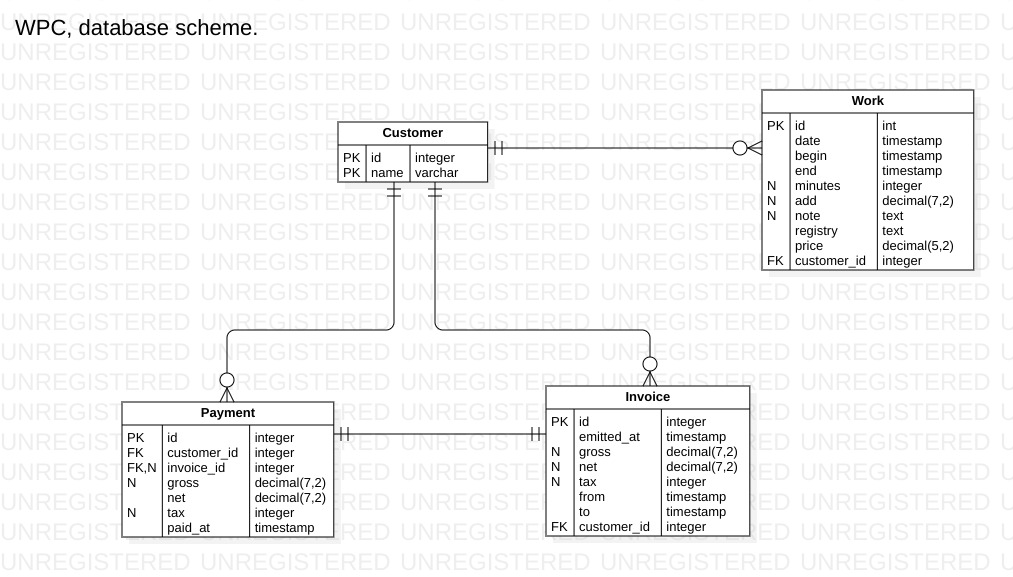
\includegraphics[scale=0.4]{wpc_data_model}

\subsection{CLI}
The command line interface is a foundamental tool: it allows the usage of the program without any complicance in UI design, however, even the CLI needs to be designed.

Commands for clients management:
\begin{lstlisting}
> cli show
> cli add <id>|<name>
> cli remove <id>|<name>
> cli switch <id>
\end{lstlisting}

Commands for work management:
\begin{lstlisting}
> (cli) work --filters column1=value1, column2=value2, ..., columnN=valueN show
> (cli) work add
> (cli) work remove <id>|<date>
> (cli) work edit <id>|<date>
\end{lstlisting}

Commands for invoices management:
\begin{lstlisting}
> (cli) inv --filters column1=value1, column2=value2, ..., columnN=valueN show
> (cli) inv add
> (cli) inv remove <id>
> (cli) inv edit <id>
\end{lstlisting}

Commands for payments management:
\begin{lstlisting}
> (cli) pay --filters column1=value1, column2=value2, ..., columnN=valueN show
> (cli) pay add
> (cli) pay remove <id>
> (cli) pay edit <id>
\end{lstlisting}

Every command will start guided procedure throught actions.

\ifdefined\COMPLETE
\else
\end{document}
\fi
